\documentclass[10pt]{article}
\usepackage[margin=1in]{geometry}

\usepackage[shortlabels]{enumitem}
\setcounter{secnumdepth}{4}


\usepackage{mathptmx}
\usepackage{graphicx}
\usepackage{times}
\usepackage{comment}
\usepackage{amstext}
\usepackage{amsmath}
\usepackage{amssymb}
\usepackage{array}
\usepackage{multirow}
\usepackage{url}
\usepackage{subfigure}
\usepackage{xcolor}
\usepackage{float}
\usepackage{slashbox}
\usepackage{pict2e}


\usepackage{fancyhdr, lastpage}
\pagestyle{fancy}
\fancyhf{}
%
\lhead{}
\chead{Fisher Rao mean bias analysis}
\rhead{}
%
\cfoot{Page \thepage{} of \protect\pageref*{LastPage}}

\usepackage{varioref}
\labelformat{equation}{(#1)}

% \usepackage{hyperref} must almost always be LAST \usepackage in
% preamble. Otherwise, you may get strange compilation errors!
\usepackage[colorlinks,linkcolor=black]{hyperref}

\begin{document}

\begin{figure}[H]
  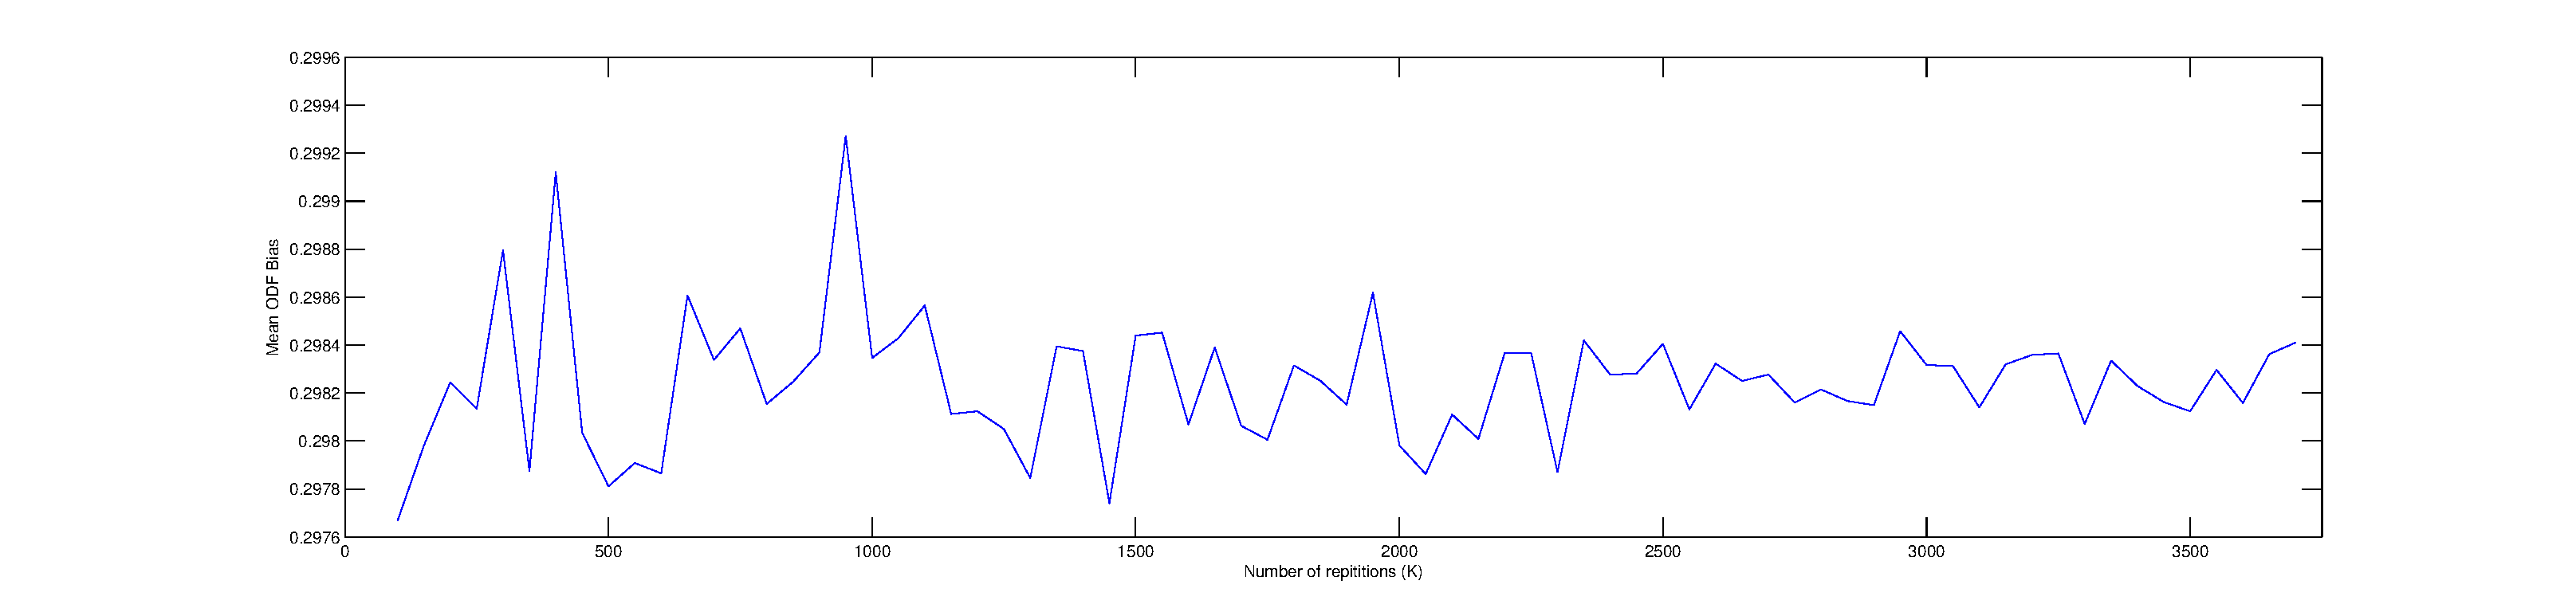
\includegraphics[width=\textwidth]{figures/mean_ODF_bias.eps}
  \caption{Mean ODF bias V.S. number of repititions $K$}
\end{figure}

\begin{figure}[H]
  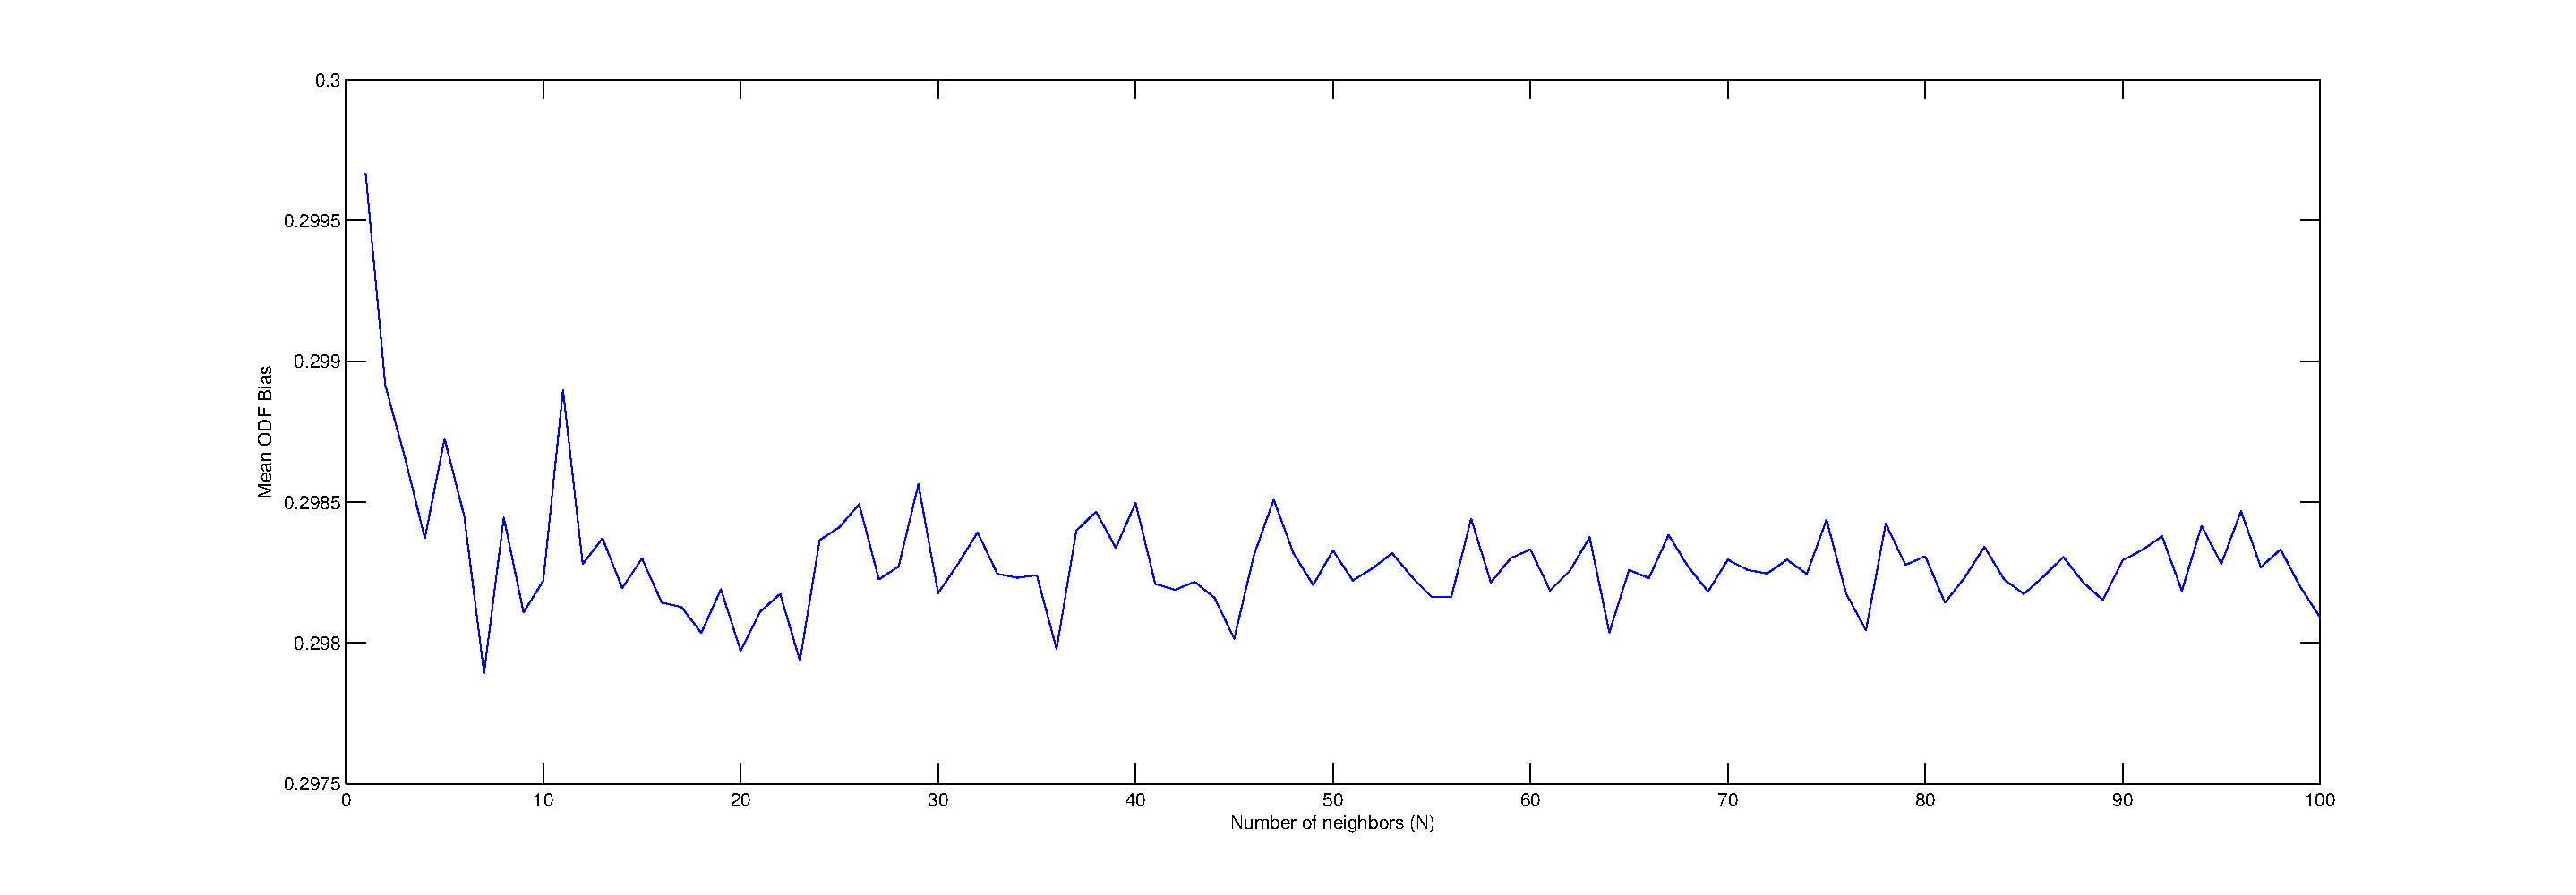
\includegraphics[width=\textwidth]{figures/neighbor_bias.eps}
  \caption{Mean ODF bias V.S. number of averaging neighbors $N$}
\end{figure}

\begin{figure}[H]
  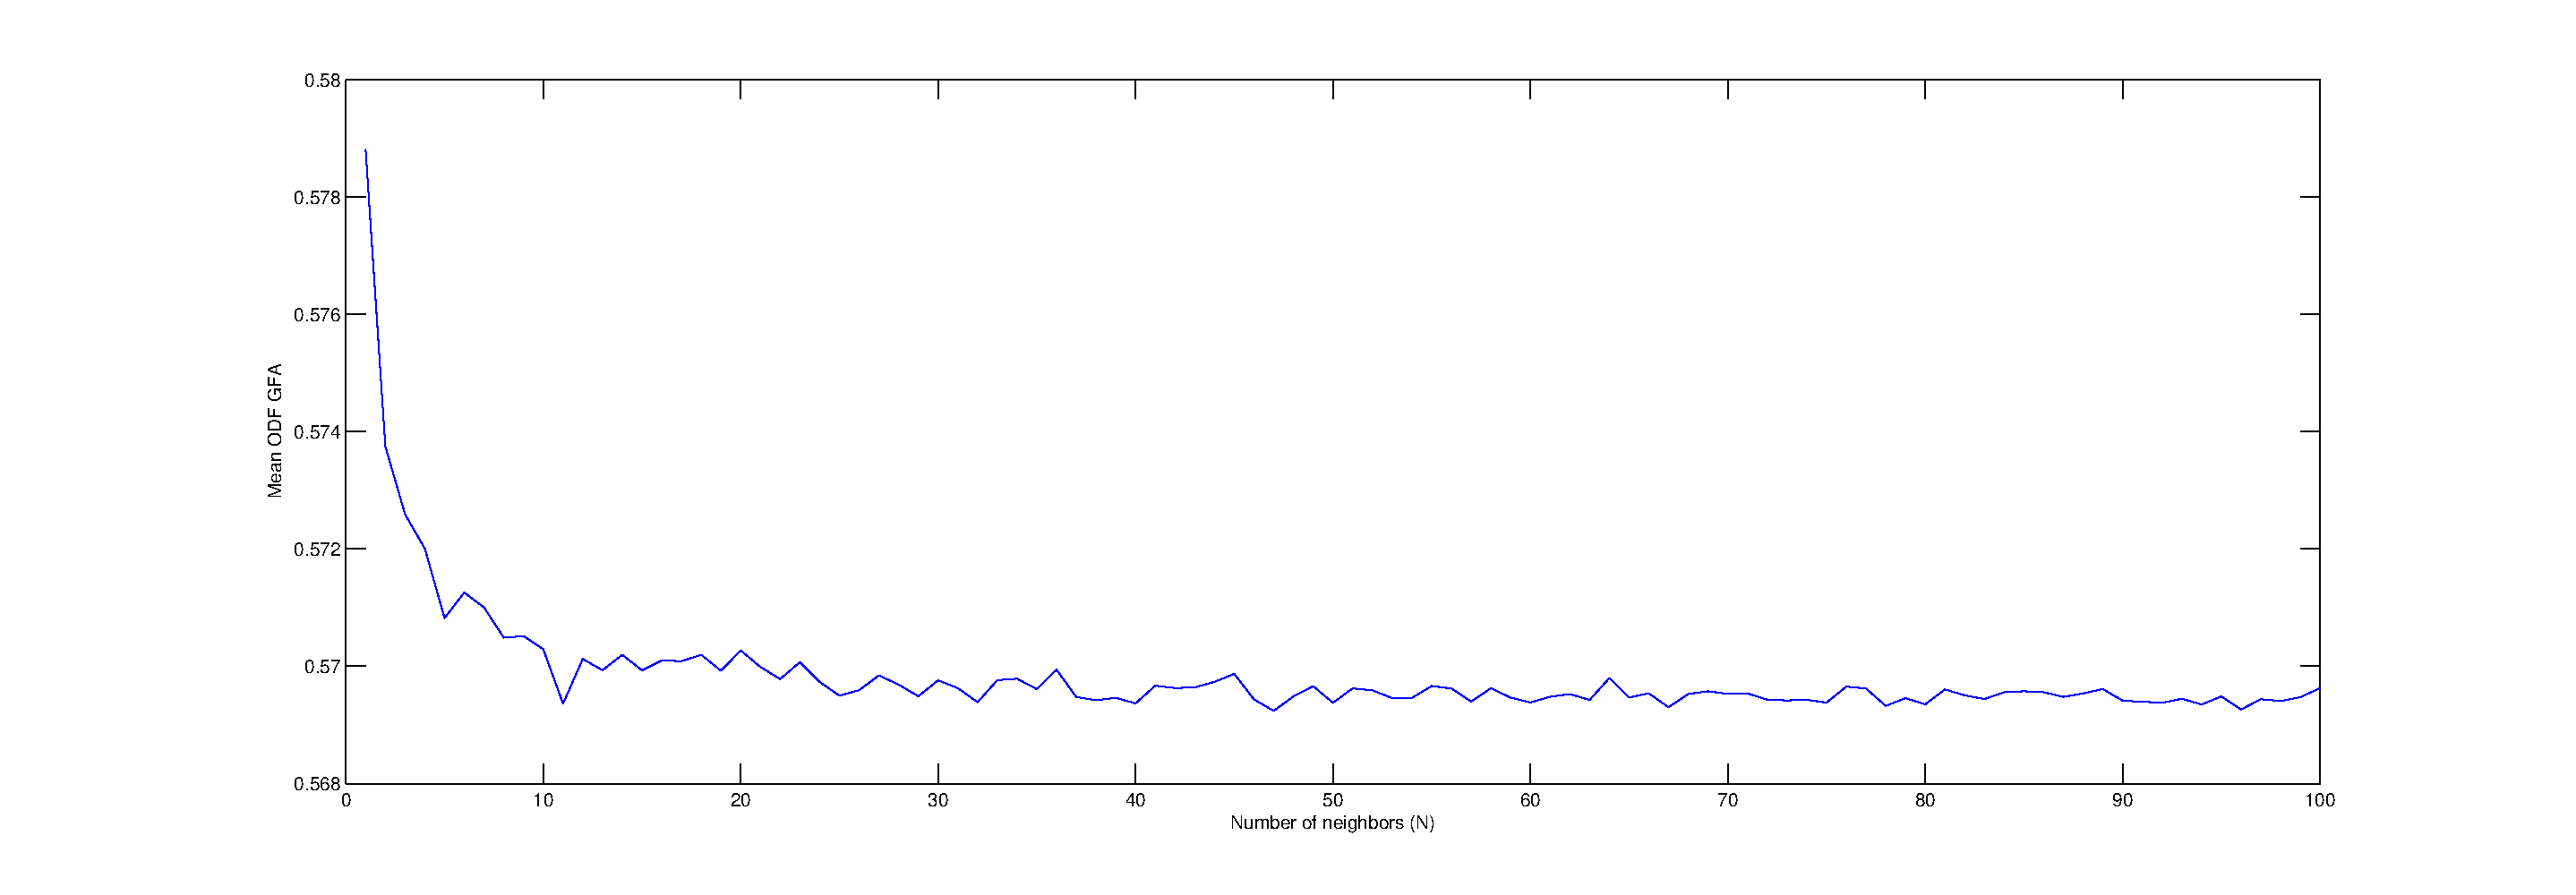
\includegraphics[width=\textwidth]{figures/mean_ODF_gfa.eps}
  \caption{Mean ODF bias V.S. number of averaging neighbors $N$}
\end{figure}

\end{document}


